\documentclass{article}
\usepackage[utf8]{inputenc}
\usepackage[dutch]{varioref}
\usepackage[autostyle]{csquotes} 
\usepackage[dutch]{babel}
\usepackage{listings}
\usepackage{pdfpages}
\usepackage{url}
\usepackage{natbib}
\usepackage{graphicx}

\title{Stageverslag}
\author{\mbox{Pieter-Jan} Robrecht}
\date{Maart 2016}

\begin{document}

%\maketitle
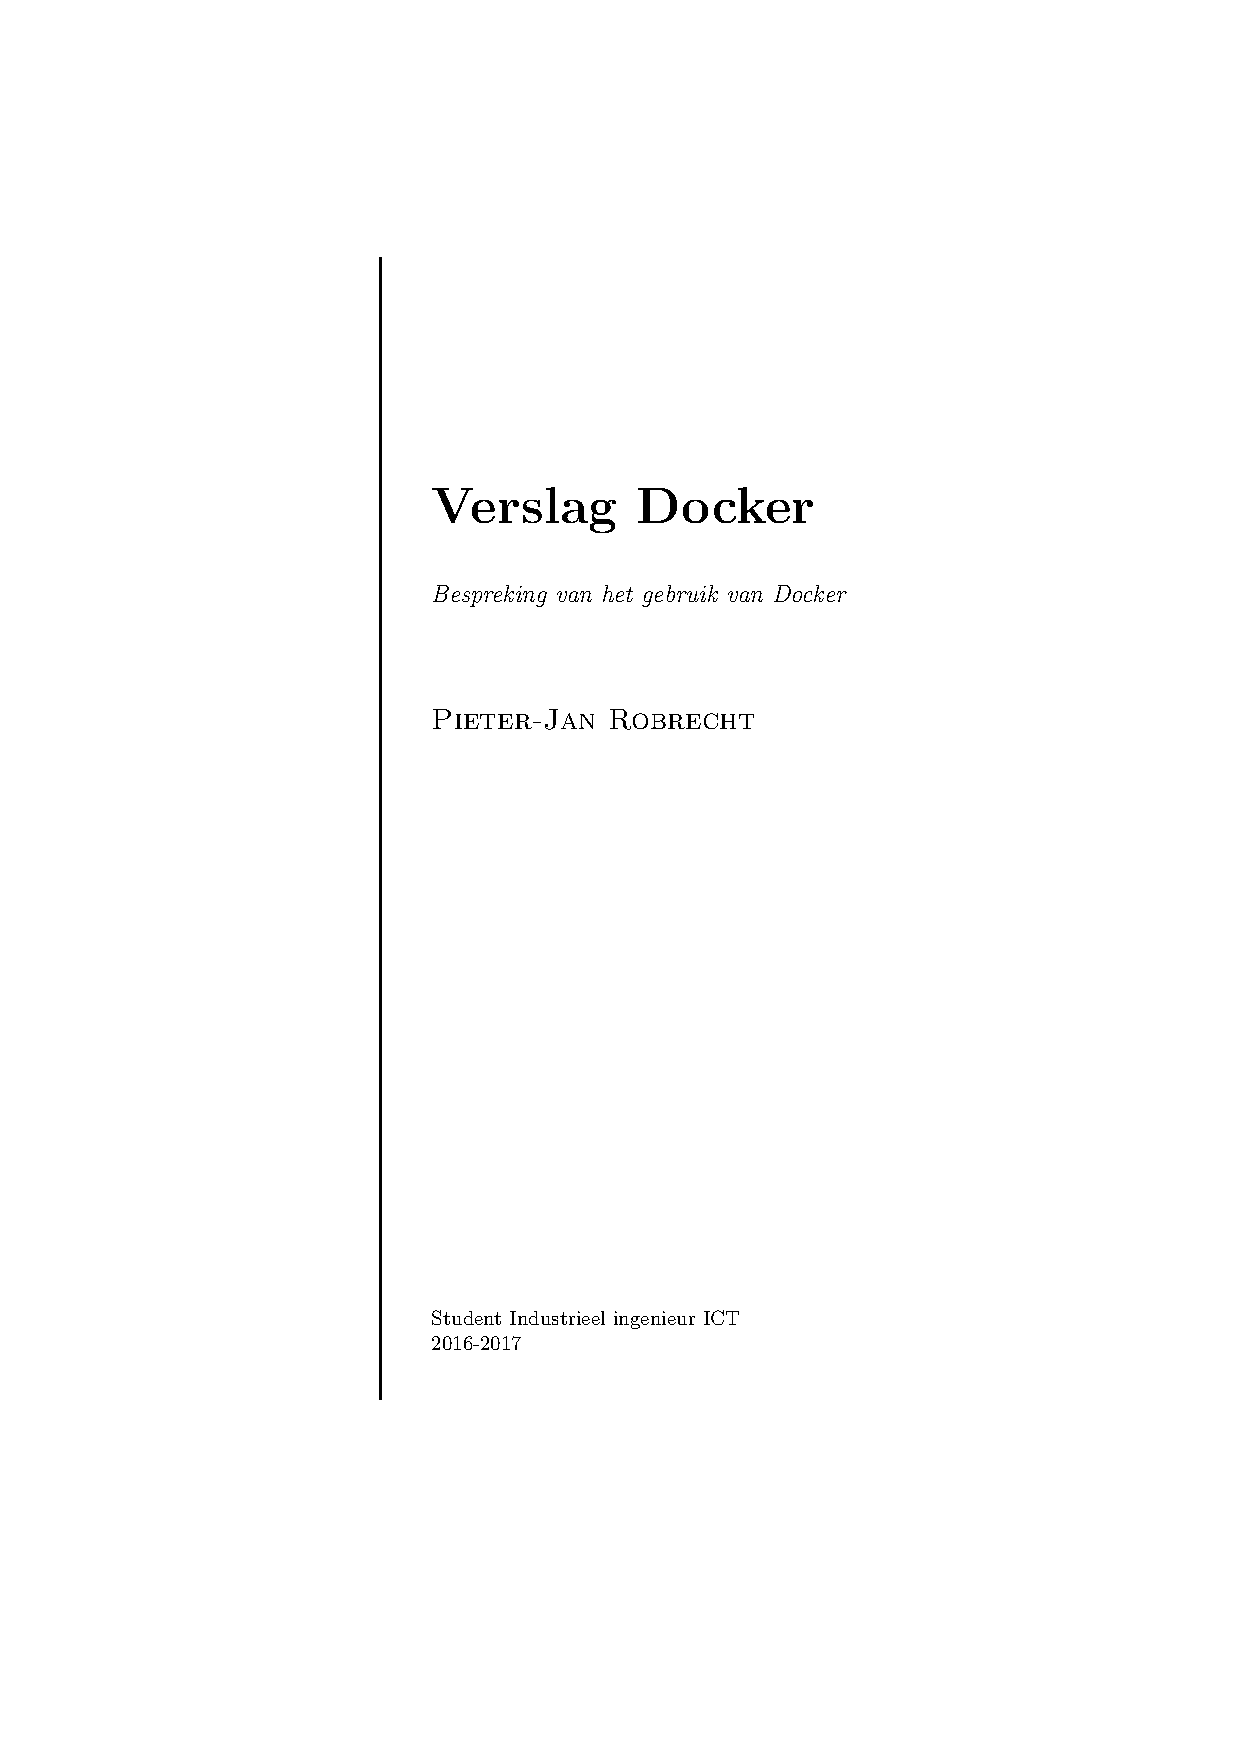
\includepdf{titel/titeldocker.pdf}

%Volgende lijn is om de titelpagina geen paginanummer te geven
\clearpage
\setcounter{page}{1}

\tableofcontents
\lstlistoflistings
\clearpage

\section{Inleiding}
Het doel van dit verslag is het bespreken van Docker als mogelijke oplossing voor het Python Installer probleem.
Voor het bespreken van Docker ging ik op een gelijkaardige manier te werk zoals tijdens mijn stage.
Ik heb de tool uitgeprobeerd en de gemaakte installer moest het volgende kunnen:
\begin{itemize}
\item het uitpakken van een zip bestand
\item het uitvoeren van de setup.py horende bij het zip bestand
\item het uitvoeren van een executable
\end{itemize}
Verder heb ik ook gekeken wat de mogelijkheden zijn voor het uitvoeren van een update.
Docker maakt gebruik van images (read-only templates met instructies) voor het opzetten van verschillende containers.
Deze containers zijn dan uitvoerbare instanties \citep{docker}.

\section{Bespreking}
Al snel blijkt dat Docker verschillende plus- maar ook minpunten heeft.
Zo is het bijvoorbeeld enkel mogelijk om Docker te installeren op een computer met Windows 10 Professional, Enterprise (Anniversary Edition) of Windows server 2016 \citep{microsoft}.
Gelukkig kon ik wel gebruik maken van de Docker toolbox waarmee ik dan aan de slag kon.
Jammer genoeg kon ik met de toolbox versie van Docker Windows containers maken.
In listing~\vref{list:dockerfile} kan u zien dat als base image Ubuntu werd gekozen.
Aangezien de base image Ubuntu is, is het niet mogelijk om Windows executables uit te voeren.
Hiernaast was het ook niet mogelijk om de setup.py uit te voeren aangezien deze geschreven is voor Windows systemen.
Het installeren en opzetten van de omgeving ging zeer vlot en verliep verder zonder problemen.


\section{Code}
\lstinputlisting[caption={Docker Dockerfile}, label={list:dockerfile}]{../code/docker/test/dockerfile.txt}

%Alfabetische volgorde
\bibliographystyle{plain}
%Orde van bib file
%\bibliographystyle{unsrt}
\bibliography{bib/dockerbib}

\end{document}